
We propose a \textit{design pattern} for building query processing systems,
with the goal of evolving query processing system's architecture from monolithic and static to modular and flexible.
Traditional static query processing systems are not able to cater to the needs of modern applications in which users and
data are geo-distributed across the globe.
Our vision is to enable query processing systems that are designed and deployed on a case-by-case basis,
with the workload characteristics, data and access distribution patterns, and requirements of specific applications in
mind.
As a first step towards this vision, we focus on the \textit{mechanisms} required for enabling a flexible and configurable
query processing system architecture.

\medskip

The key idea for the proposed design pattern \textit{assembly-based modularity}.
The query processing system's architecture is modular:
it is constructed by interconnecting composable building blocks
that encapsulate components of a traditional query processing system such as indexes, materialized views,
and caches, as well as relational operators such as filters, aggregations, and joins.
Modularity translates design decisions about the use of derived state to which building blocks are used and how they are
interconnected.
For example, adding a caching layer to an existing system can be done by extending an existing query system architecture
with additional building blocks.

Moreover, modularity enables configurable placement.
The components of a modular architecture, as opposed to a monolithic one,
can be decoupled from the storage tier, and flexibly placed across the system infrastructure.


\section{Overview: a modular query processing architecture}

According to the design pattern that we propose,
a query processing system is a composition of building blocks that encapsulate query processing tasks, called
Query Processing Units (QPUs).

A QPU is a \textit{system component} that combines properties of a microservice and a streaming operator.
Similarly to a streaming operator, a query processing unit receives one or more input streams,
performs a computation over these streams, and emits an output stream.
Similarly to microservice, a QPU exposes an interface for receiving query requests.
The response to query request is a stream.
Moreover, a QPU can send query request to other QPUs.
Therefore, every input stream is the output stream of another QPU, and every output stream is the response to a query request.

\medskip
\noindent
A query processing unit can implement a \textit{relational operator}.
For example, a ``join operator'' QPU receives input streams that represent the tables to be joined,
and emits an output stream that represents the results of the join operation.

Moreover, a QPU can implement a \textit{derived state structure}, such as an index, a materialized view, or a cache.
For example, a ``secondary index'' QPU receives an input stream that represents notifications for updates to the table
to be attribute to be indexed; it maintains a secondary index data structure, which it stores as internal state.
When it receives a query request, it reads from its internal state and emits the result as an output stream.

Finally, multiple ``secondary index'' QPUs can be used to implement partitions of \textit{partitioned index}
Another type of QPU can be then used to as a ``partition manager''; given a query, the ``partition manager'' QPU sends query
requests to the appropriate  ``index partition'' QPUs, thus initiating input streams; it then combines these input streams
and emits the result as an output stream.

Our key insight all three of the described QPU types --- relational operators, derived state, and routing operators ---
can be generalized to a system component with common semantics, and thus can be composed arbitrarily to implement complex
query processing computations.

\medskip
\noindent
QPUs are organized in a directed acyclic graph.
The edges of the graph represent potential query request - response steam relations.
For example, an edge from $QPU_a$ to $QPU_b$ indicates that $QPU_a$ can send query requests (and therefore establish input streams)
to $QPU_b$.
We call $QPU_b$ a \textit{downstream} or \textit{outwards} connection of $QPU_a$.
Base data are the leaves of the graph (nodes with only incoming edges),
and client queries enter the graph through its root nodes (nodes with outgoing edges).

When a QPU receives a query, it can process it by reading from its internal state, it can initiate input streams
by sending query requests to its some of its downstream connections and produce query results using these streams,
or a combination of the two.
This process is recursively performed at each downstream QPU, creating a query execution tree.

\section{Query Processing Unit: the building block}

\subsection{The Query Processing Unit abstraction}

The key property required by query processing unit to effectively serve as building blocks of the modular query
processing systems is composability:
QPUs should be able to be interconnected in various topologies, and interoperate in the execution of query processing tasks.

To achieve this, we define a common set of properties that any query processing unit should conform to.
This properties include a common interface for receiving query request, and common the interaction semantics among QPUs.
We call this set of properties the query processing unit \textit{abstraction}.
Using object-oriented programming terminology, the QPU abstraction can be viewed as an \textit{abstract class}
that defines a set of methods, but does not include their implementation.
Implementations of the QPU abstraction define \textit{QPU classes} with specific functionalities,
such as join or index QPU classes.
Using the object-oriented programming analogy, QPU classes can be viewed as classes that implement the QPU
abstract class.
Finally, specific \textit{QPU instances} can be viewed as objects of a specific QPU class, for example a index QPU that
indexes the attribute $predominantColor$ of a table $photoAlbum$.
The building blocks of a modular query processing system are QPU instances.

In the rest of this thesis we use the terms query processing unit, QPU, and unit interchangeably to refer to QPU instances.

\bigskip

More specifically, the query processing unit abstraction defines a \textit{system component} with the following properties:

\begin{figure}[t]
  \centering
    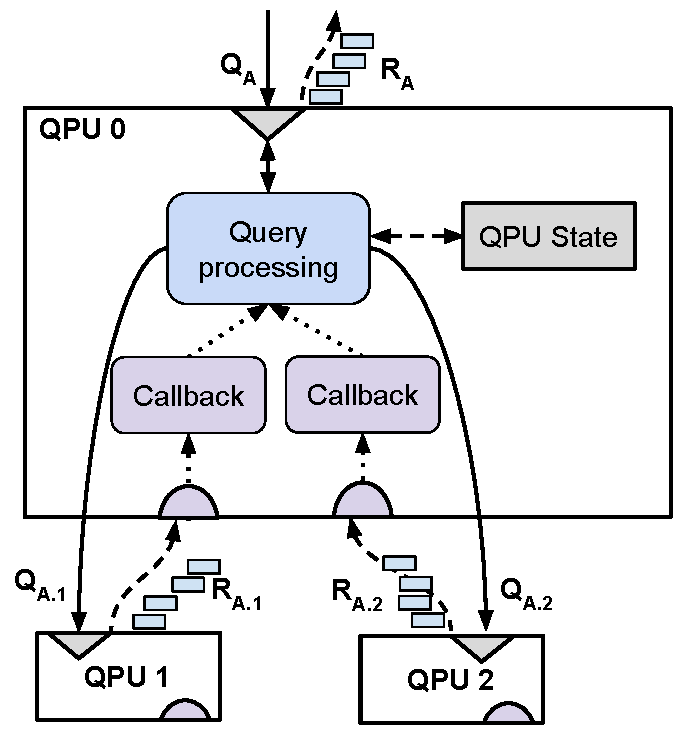
\includegraphics[width=0.5\textwidth]{./figures/design_pattern/qpu_abstraction.pdf}
  \caption{A conceptual depiction the QPU abstraction.}
  \label{fig:qpu_abstraction}
\end{figure}

\medskip
\noindent
\textbf{Query interface.}
Every QPU exposes an interface for receiving query requests.
While this interface is common among all QPUs, QPU classes and specific QPU instances restrict the set of queries
that they can serve.
For example, a QPU may only serve queries about a specific database table.
As a result, QPUs can be though of as microservices that serve queries

The QPU's query interface has \textit{streaming semantics}.
An invocation of the interface establishes between the QPU and caller:
the QPU sends query result entries as stream records; the caller can send control messages such as acknowledgements.
We present the query interface in more detail in section \todo{ref}.

The query interface can be invoked by other query processing units.
This is how QPUs interoperate and forms the basis of the query processing system's computation model \todo{ref}.
We call the act of a $QPU_a$ invoking the query interface of a $QPU_b$, a \textit{downstream query}.

\medskip
\noindent
\textbf{Query processing function.}
Every QPU implements a function that is called when its query interface is invoked, and is responsible for processing
the given query and writing to the query result stream.

The implementation of this computation is specific to each QPU class.

Two capabilities are available for the implementation of the query processing function:
accessing the QPU's state, and initiating input streams by sending query requests to downstream connections.

\medskip
\noindent
\textbf{State.}
Each QPU maintains \textit{internal} state, that is accessible only by that specific QPU.

We distinguish the QPU state in three parts according to its functionality.
In this section, we present an overview of the functionality of each state type.
In section~\ref{ref:specification} we present the QPU's state in detail.

Each query processing unit maintains \textit{configuration state} that represents the query processing unit's
configuration parameters.

In addition, each QPU with outwards connections in the QPU graph maintains information about the
\textit{query processing capabilities} of these QPUs. \todo{ref}.
This information is used by the for creating and generating and sending downstream query requests in order to initiate
input streams that it can use during query processing \todo{ref}.

Finally, query processing units that implement derived state structures, and units need to store intermediate query processing
results, for example \todo{in streaming join computation?}, maintain \textit{query processing state}.

\medskip
\noindent
\textbf{Input stream callback function.}
Each QPU implements a callback function that is called for each record received through an input stream.
Similarly to the query processing function, the implementation to callback function is part of the definition of each
QPU class.

\bigskip

A conceptual depiction of the query processing unit abstraction is shown in Figure~\ref{fig:qpu_abstraction}.
When the QPU's query API is called, a response stream ($R_A$) is established between the unit and the client, and
the unit's query processing computation is invoked.
The query processing computation can read the QPU's state, and can perform downstream queries to other units.
For each downstream query, a corresponding stream is established ($Q_{A.1}$ and $Q_{A.2}$).
When a record is received from one of the streams, the QPU's callback computation is invoked.
Each callback computation processes the received record, and returns the result to the query processing computation.
Upon receiving a result from the callback, the query processing computation can write to the QPU's
state and potentially send a computed query result through the response stream.


\subsection{Query Processing Unit specification}
\label{ref:specification}

In this section we present the detailed specific of the Query Processing Unit abstraction.

\subsubsection{Query interface}

In this section, we first present a high level overview of the QPU abstraction's interface,
and then describe each of its elements in more detail.

Each query processing unit exposes and interface for receiving query requests:


\begin{displaymath}
  Query(QueryRequest) \rightarrow QueryResponse
\end{displaymath}

$QueryRequest$ specifies a predicate on the data items' \textit{attributes}, and a \textit{time interval}.

$QueryResponse$ is a stream containing records that represent \textbf{updates} (an update can be a creation, modification, or deletion)
performed to data item of the corpus
It represents updates as \textit{deltas}:
a delta representing an update $u$ contains the data item's attribute values before $u$ is applied,
and those after the $u$ is applied.

More specifically:
\[
  QueryResponse = [UpdateDelta]
\]
where
\[
  UpdateDelta =
\]
\[
  (DataItemID, [(AttributeName, AttributeValue_{old}, AttributeValue_{new})], timestampValue)
\]
\todo{ensure consistent terminology}

An $update$ is a triplet containing
(1) the primary key of the data item ($DataItemID$) it refers to,
(2) a list of triplets of the form $(AttributeName, AttributeValue_{old}, AttributeValue_{new})$ that represent the
data item's attribute values before and after the update is applied,
and (3) the timestamp ($timestampValue$) assigned to the update.

Given a $QueryRequest$ that specifies an attribute predicate $Pred$ and a time interval $T$ $=$ $[t_1, t_2)$
\begin{itemize}

  \item If $t_1$ $=$ $t_2$ = $t$,
  then for each data item $QueryResponseRecord$ contains \textit{only the latest update before $t$},
  provided that after applying that update the data item's attributes satisfy $Pred$.
  We term this case a \textit{snapshot query}.

  \item if $t_1$ $<$ $t_2$,
  then for each data item $QueryResponseRecord$ contains any update with $t_1$ $\leq$ $timestampValue$ $<$ $t_2$,
  provided that the data item's attributes satisfy $Pred$ \textit{either before or after applied that update}.
  We term this case a \textit{an interval query}.

\end{itemize}

A snapshot query, therefore queries a \textit{snapshot} of the corpus that contains the effect of every update with a
timestamp $<$ $t$.
By returning the latest update before $t$, a snapshot query effectively returns that \textit{state} of the data items
that satisfy $Pred$ in the snapshot defined by $t$.

In contrast, an interval query receives for each data item any update within the specified time interval that modifies
the data item so that either is starts of it stops satisfying $Pred$.
By using a $t_2$ in the future, an interval query can continue receiving updates that satisfy $Pred$.
This provides a mechanism for \textit{subscribing to notification for updates based on a given predicate}.

\bigskip

\textbf{Query Language.}
% https://documentation.basis.com/BASISHelp/WebHelp/usr2/sql_grammar.htm
% http://www.h2database.com/html/grammar.html#expression
% $Query$ receives $QueryRequest$ and returns a stream of $QueryResponseRecord$:

The query processing abstraction implements an SQL-like query language,
that supports point and range queries, logical operators, aggregation functions, and joins.

We argue that these is no inherent limitation in the query processing unit abstraction that prevents it from implementing
more complex functionalities, such as nested queries.
However, we consider additional functionalities to be out of the scope of this work.
We believe this query language can effectively demonstrate that the query processing unit abstraction can be used as building
block for constructing fully-functional query processing systems.

The QPU abstraction's query language has following syntax:

{\obeylines\obeyspaces
\texttt{
QueryRequest          ::=  SELECT SelectExpression
~~~~~~~~~~~~~~~~~~~~~~~~~~~FROM TableExpression
~~~~~~~~~~~~~~~~~~~~~~~~~~~WHERE PredicateExpression
~~~~~~~~~~~~~~~~~~~~~~~~~~~TIMESTAMP TimestampExpression \todo{the timestamp can be just another attribute, but I think we need to have it separate for emphasis}
~~~~~~~~~~~~~~~~~~~~~~~~~~~[ GROUP BY attributeName ]
~~~~~~~~~~~~~~~~~~~~~~~~~~~[ ORDER BY OrderByExpression \{ ASC | DESC \} ]
}}

{\obeylines\obeyspaces
\texttt{
SelectExpression      ::=  ALL
~~~~~~~~~~~~~~~~~~~~~~~~~~~SelectExpressionItem , SelectExpression |
~~~~~~~~~~~~~~~~~~~~~~~~~~~SelectExpressionItem
}}

{\obeylines\obeyspaces
\texttt{
SelectExpressionItem  ::=  SUM(attributeName) | AVG(attributeName) |
~~~~~~~~~~~~~~~~~~~~~~~~~~~MAX(attributeName) | MIN(attributeName) |
~~~~~~~~~~~~~~~~~~~~~~~~~~~attributeName
}}

{\obeylines\obeyspaces
\texttt{
TableExpression       ::=  tableName JoinType tableName USING attributeName |
~~~~~~~~~~~~~~~~~~~~~~~~~~~tableName
}}

{\obeylines\obeyspaces
\texttt{
JoinType              ::=  \{ INNER | \{ LEFT | RIGHT \} OUTER \} JOIN
}}

{\obeylines\obeyspaces
\texttt{
PredicateExpression   ::=  PredicateExpression OR PredicateExpression |
~~~~~~~~~~~~~~~~~~~~~~~~~~~PredicateExpression AND PredicateExpression |
~~~~~~~~~~~~~~~~~~~~~~~~~~~NOT PredicateExpression |
~~~~~~~~~~~~~~~~~~~~~~~~~~~Term Op Term
}}

{\obeylines\obeyspaces
\texttt{
Term                  ::=  attributeName | Value
}}

{\obeylines\obeyspaces
\texttt{
Op                    ::= > | >= | < | <= | = | !=
}}

{\obeylines\obeyspaces
\texttt{
Value                 ::= stringValue | floatValue | intValue |
~~~~~~~~~~~~~~~~~~~~~~~~~~dateTimeValue | timestampValue
}}

{\obeylines\obeyspaces
\texttt{
OrderByExpression     ::= attributeName , OrderByExpression |
~~~~~~~~~~~~~~~~~~~~~~~~~~attributeName
}}

{\obeylines\obeyspaces
\texttt{
TimestampExpression   ::= FROM TimestampTerm [ TO TimestampTerm ]
}}

{\obeylines\obeyspaces
\texttt{
TimestampTerm         ::= SYSTEM START | LATEST | timestampValue
}}

~ \bigskip

In practice, each QPU class can only process a subset of the queries that can be expressed by this query language,
according to its functionality.
For example, a QPU class that implements a join operator can perform a only join over two input streams.
Performing an aggregation or applying a predicate over the result of the join requires this use of other QPU classes.

\todo{references: QPU classes, composition / query execution}

Moreover, individual QPUs of a certain class may support different subsets of the query language according to their
configuration.
For example, two instances of a filter operator QPU class may provide predicate queries for different tables.

% % ---- QPUs are able to send query requests to other units (their child nodes in the QPU graph) by invoking their API.

\subsubsection{QPU State}

A query processing unit maintains the following types of state:

\medskip
\noindent
\textbf{Query processing state}
The QPU's query processing state can be used to implement derived state structures, such as indexes, materialized views and
caches.
In addition it can be use for storing intermediate state used in query processing computations.

We model the query processing state as ordered key/value map, in which keys are string values, and values are lists of
data items, represented as:
\[
  (DataItemID, [(AttributeName, AttributeValue)], timestampValue)
\]

Using pseudocode, we can represent the query processing state as follows:

\begin{lstlisting}[caption={Pseudocode for the QPU's query processing state},captionpos=b,label={lst:qpustate}]
type DataItem {
  dataItemID  string
  attributes  [(AttributeName, AttributeValue)]
  ts          timestamp
}

class QueryProcessingState
  function Get(Key_low, Key_high) [(Key, [DataItem])]
  function Put(Key, [DataItem])
\end{lstlisting}

$Get$ retrieves the query processing state entries with $Key_low$ $<$ $key$ $\leq$ $Key_high$.
$Put$ modifies the value of the query processing state for a given key.
It can be used with a non-existing key to create a new entry, or with an empty value to delete an entry.

\medskip
\noindent
\textbf{Configuration state.}
The configuration state represents the configuration parameters passed to a query processing unit when it is created.

The configuration state consists of two types parameters:
\begin{itemize}
  \item Connection parameters.
  The QPU configuration specifies the endpoints of the unit's downstream connections in the QPU graph.

  \item Class-specific parameters.
  Instances of a QPU class can have different properties.
  For example, different instances a QPU class that implements a query cache can have different cache sizes.
  These characteristics are defined by the QPU's class-specific configuration.

\end{itemize}
% % This is the part of the state that defines the QPU's behavior (includes its type
% % and neighborhood).
% % Passed as argument during initialization.
% % This type of state is composed of configuration parameters, such as the endpoint of its downstream neighbors.

\begin{lstlisting}[caption={Pseudocode for the QPU's configuration state},captionpos=b,label={lst:qpuconfigstate}]
class ConfigurationState
  function GetConfigParameter(Key) ConfigParameterValue
\end{lstlisting}

\todo{..}

\medskip
\noindent
\textbf{Local graph view.}
% This is the part of the state that describes the QPU's knowledge/view of the
% sub-graphs it is connected to.
% It is initialized using the ``getConfig'' API method.
% Each QPU maintains metadata that represent information about its downstream neighbors, such as their QPU class,
% and their capabilities \todo{ref}.
% These metadata is used during query processing for generating downstream query requests \todo{ref}.

%  shemata
%  example with join
\todo{..}

\subsubsection{Query processing function}

% % \begin{algorithm}
% % \caption{Query processing function signature}
% % \label{func:query_processing}
% % \begin{algorithmic}
% % \Function{ProcessQuery}{QueryRequest, State, DownstreamNeigbors, ResponseStream}
% % \end{algorithmic}
% % \end{algorithm}
% Every QPU implements a function that is responsible for processing queries request received by the QPU.
% The query processing function is the core to the query processing unit's functionality.
% As different QPU classes have implement different functionalities, the query processing function's implementation is
% class-specific.


\begin{lstlisting}[caption={Query processing function signature},captionpos=b,label={lst:query_processing_func}]
function ProcessQuery(QueryRequest, State, DownstreamConnections, ResponseStream)
\end{lstlisting}

\noindent
Listing~\ref{lst:query_processing_func} shows the query processing function's signature.
$ProcessQuery$ receives the following arguments:
\begin{itemize}

  \item $QueryRequest$, which represent the received query request.
  \item $State$, which allows $ProcessQuery$ to access QPU's state.
%   Listing~\ref{lst:state_object} blah

%     \begin{lstlisting}[caption={The QPU's $State$ object},captionpos=b,label={lst:state_object}]
%     type State {
%       qpState                 QPState
%       config                  Configuration
%       downstreamCapabilities  map[downstreamQPU]Capabilities
%     }

%     type DataItem {
%       dataItemID  string
%       attributes  [(AttributeName, AttributeValue)]
%       ts          timestamp
%     }

%     function (QPState) Get(Key_low, Key_high) [(Key, [DataItem])]
%     function (QPState) Put(Key, [DataItem])

%     function (Configuration) GetConfigParameter(Key) ConfigParameterValue

%     \end{lstlisting}


  \item aaa
\end{itemize}


% % The query processing function's implementation is specific to each QPU class
% % the given query and writing to the query result stream.

% The implementation of this computation is specific to each QPU class.

% Two capabilities are available for the implementation of the query processing function:
% accessing the QPU's state, and initiating input streams by sending query requests to downstream neighbors.


% \subsubsection{Input stream callback function}

% Each QPU implements a callback function that is called for each record received through an input stream.

% ... The implementation of this computation is may differ between QPU classes ...

% % \begin{algorithm}
% % \caption{Input stream callback function}
% % \label{func:callback}
% % \begin{algorithmic}
% % % \Function{ProcessQuery}{QueryRequest, State, DownstreamNeigbors, ResponseStream}
% % \end{algorithmic}
% % \end{algorithm}

\subsection{QPU classes}
\label{sec:qpu_classes}

As described in the previous section, the query processing unit abstraction has the role of ``template'',
defining unified semantics that every QPU conforms with.
This ensures that query processing units can be arbitrarily interconnected and interoperate to implement query processing
tasks.

A QPU class is an \textit{instantiation} of the query processing unit abstraction, which defines implementations for
the \textbf{query processing function} and the \textbf{input stream callback function}.

In this section, we present a categorization of QPU classes according to their general characteristics,
and demonstrate some specific examples of QPU classes.
We intentionally do not present a more extended list of QPU classes as it is out of the scope of this chapter.
We present additional QPU classes in chapters~\ref{ch:case_studies}, \ref{ch:proteus}, \ref{ch:evaluation}.

We categorize QPU classes in three groups, according to their general characteristics:
\begin{itemize}
  \item \textbf{Relational operator QPUs}.
  Classes in this group can be viewed as \textit{streaming relational operators}.
  They receive input data streams and perform filtering or transformation of these streams.
  Every input stream record, results in the QPU emitting zero or one records in the output stream.

  Conforming to the QPU specification, every input stream is the output stream of another QPU,
  and every output stream is the response to a query request.

  Some examples QPU classes in this group are:
  \begin{itemize}
    \item \textbf{Filter:}
    A filter QPU implements a streaming filter operator.
    \todo{more details in example}
    \item \textbf{Join}:
    A join QPU implements a streaming join operator.
    Given a query with a join operator,
    the join QPU is responsible for initiating input streams by sending the appropriate query requests to downstream QPUs,
    performing a streaming join operation on the input streams, and emitting the result at its output stream.
    \item \textbf{Aggregator}:
    An aggregator QPU implements a aggregation function over an input stream, such as count, sum, average, min or max.
    The aggregator QPU emits an record at the output stream for each input record that changes the aggregation value.
  \end{itemize}

  \item \textbf{Derived state QPUs}.
  Classes in this group implement derived state structures, such as indexes, caches, and materialized views.

  QPU classes of this group make use of the same use of the ``query request - output stream'' semantics to implement
  their functionality:
  \begin{itemize}
    \item \textbf{Secondary index and Materialized View:}
    An secondary index (or materialized view) QPU initiates an input steam by sending a query request with an \textit{interval query without
    an upper bound timestamp}.
    In that way, the QPU effectively \textit{subscribes to notifications} for updates to the corpus.

    For each input record, the QPU's callback function updates the QPU's query processing state accordingly.
    When receiving a query request, the unit computes the results by reading from its query processing state,
    and emits them to the output stream.

    For simplicity we assume that a secondary index QPU maintains an index for a single attribute
    (and the same for materialized view QPUs respectively).

    % discussion: input output disconnected here
    \item \textbf{Cache:}
    A cache QPU stores query results at its query processing state.
    When receiving a query request, the QPU's query processing function first determines it has stored the query result,
    and if yes it retrieves and emits it at the output stream.
    Alternatively, the query processing function sends query request at a downstream connection, forwarding the same query.
    The callback function the stores each received record at the query processing state, and then emits it at the output
    stream.
    \end{itemize}

  \item \textbf{Routing QPUs}.
  Classes of this group are responsible for implementing higher level functionalities, such as coordinating partitioned or
  replicated derived data structures, or performing load balancing.

  Examples of classes in this group include:
  \begin{itemize}
    \item \textbf{Partition manager:}
    A partition manager QPU is responsible for managing access to set of QPUs that implement index or materialized view
    partitions.
    The unit has outgoing edges in the QPU graph to a number of partitions.
    It also maintains at its connection's capabilities state information about the partitioning scheme and the portion of
    the partitioned space that each of its connections corresponds to.

    When receiving a query request, the QPU's query processing function uses these information to determine which
    partitions need to be contacted for the given query,
    and sends query requests to the corresponding downstream connections.
    The QPU then combines the resulting input streams and emits the combined stream as its output stream.

    \item \textbf{Load balancing and replica manager:}
    QPUs of these classes have similar functionalities with the partition managers:
    given a query they select the most suitable among their downstream connections, according to a certain criterion specific
    to each class, forward the given query, and finally forward the resulting input stream to their output stream.

    \end{itemize}

  \item \textbf{Database driver QPUs}
  The database driver class is responsible for connecting the QPU graph with the corpus.
  It is particular class, as database driver QPU do not support downstream connections to other QPUs.
  As a result they are located at the leaves of the QPU graph.

  Database driver QPUs apply a restriction on the query language.
  Their query interface supports queries of the form:
  {\obeylines\obeyspaces
  \texttt{SELECT SelectExpression from TableName TIMESTAMP TimestampExpression}}

  Given a query, the query processing function uses the interface and mechanisms of they corpus database in order to generate and emit
  the output stream.

  Database driver QPUs acts as wrappers that expose a common interface and semantics --- those defined by the QPU abstraction --- to the
  QPU graph, independent of how the corpus is stored and accessed.

  As a result database driver classes are database-specific.
  QPU-based query processing systems are compatible with any corpus database as long as there is a corresponding database driver class
  to provide the interface with that database.
\end{itemize}

\subsubsection{QPU class case studies}

\textbf{Filter}

\bigskip
\noindent
\textbf{Secondary index}


\section{QPU-based query processing systems}


\subsection{Query processing system architecture}

\begin{figure}[t]
  \centering
    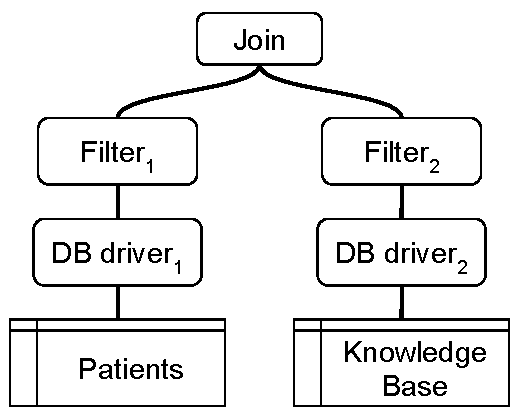
\includegraphics[width=0.4\textwidth]{./figures/design_pattern/qpu_graph_emergent_properties.pdf}
  \caption{QPU graph example}
  \label{fig:qpu_graph_emergent_properties}
\end{figure}

A \textit{QPU-based} query processing system is a directed acyclic graph (DAG).
Graph nodes are query processing unit instances.
Edges represent potential query request - response steam relations between QPUs.
A directed edge from $QPU_a$ to $QPU_b$ indicates that $QPU_a$ can send query requests to $QPU_b$.
When $QPU_a$ sends a $QPU_b$ a query request to $QPU_b$, a stream of query results with the opposite direction is established between them.

Leaf nodes (nodes with no outgoing connections) are always database driver QPUs.
Queries enter the QPU graph through root node (nodes with no incoming connections).
\todo{ref}

The capabilities of a QPU-based query processing system are emergent from the functionalities of the QPUs at its node, as well as the
graph topology.
For example, consider the QPU graph depicted in Figure~\ref{fig:qpu_graph_emergent_properties}:
\begin{itemize}

  \item $DB$ $driver_1$ can process queries with the form:
  {\obeylines\obeyspaces
  \texttt{SELECT SelectExpression from Patients TIMESTAMP TimestampExpression
  }}
  where $SelectExpression$ can contains one or more attributes of the $Patients$ table.

\item $DB$ $driver_2$ can process queries with the form:
{\obeylines\obeyspaces
\texttt{SELECT SelectExpression FROM KnowledgeBase TIMESTAMP TimestampExpression
}}
where $SelectExpression$ contains one or more attributes of the $KnowledgeBase$ table.

\item $Filter_1$ can send downstream queries to $DB$ $driver_1$
and apply a filter to its input stream.
Therefore, $Filter_1$ can process queries of the form:
{\obeylines\obeyspaces
\texttt{SELECT SelectExpression FROM Patients
        WHERE PredicateExpression
        TIMESTAMP TimestampExpression
        }}
where $SelectExpression$ and $PredicateExpression$ can use attributes of the $Patients$ table.

\item Similarly, $Filter_2$ supports queries of the form:
{\obeylines\obeyspaces
\texttt{SELECT SelectExpression FROM KnowledgeBase
        WHERE PredicateExpression
        TIMESTAMP TimestampExpression
        }}
where $SelectExpression$ and $PredicateExpression$ can use attributes of the $KnowledgeBase$ table.

\item $Join$ can send downstream queries to $Filter_1$ and $Filter_2$
and join the two input streams based on a given attribute.
Assuming that the $Patients$ and $KnowledgeBase$ tables have a common attribute, $symptoms$,
$Join$ can process queries of the form:
{\obeylines\obeyspaces
\texttt{SELECT SelectExpression
        FROM Patients JOIN KnowledgeBase ON Patients.symptoms = KnowledgeBase.symptoms
        WHERE PredicateExpression
        TIMESTAMP TimestampExpression
        }}
where $SelectExpression$ and $PredicateExpression$ uses attributes from both tables.

\end{itemize}

\todo{ref}

\subsubsection{QPU-graph topology rules}
topology cannot be arbitrary

rules that stem from the query processing units' functionalities

non-exhaustive list,
For each QPU class can be generalized to two types of rules:
(1) number of downstream connections, and (2) the \textit{query processing capabilities} of the downstream connection

\begin{itemize}
  \item All QPU graphs mush have database driver QPUs as their leaves.
  Database drivers generate the initial streams that any other QPU builds on.

  \item Most QPUs in the relational operator and derived state groups must have a single downstream connection.
  Exception consists relational operator QPUs that by definition operate on more that one input streams, such as join QPUs.

  \item A materialized view QPU must have a downstream connection that can provide a stream of updates on the query
  that defines the materialized view
  In more detail, the downstream connection of a materialized view QPU must be the root of a subgraph that
  \begin{itemize}
    \item Can process the query the is the materialized view's definition.
    \item Supports \textit{interval queries} on that query.
  \end{itemize}
  \todo{use existing example}

  \item Similarly, a secondary index QPU must have a downstream connection that can provide a stream of updates on the
  attribute that QPU is configured to index.

  \item A cache QPU must have at least on downstream connection.
  This connection can be towards any valid sub-graph.

  \item Similarly, a filter QPU can be connected to any valid sub-graph.

  \item A partition manager QPU must have one or more downstream connections to derived state QPUs that implement
  partitions of a derived state structure.
  In more detail:
  \begin{itemize}
    \item All downstream connection must be of the same QPU class

    \item They must be configured as partitions of a logical global derived structure, based on a single partitioning key.
  \end{itemize}

  \item A load balancer QPU must have one or more downstream connections, and the \textit{intersection} of the queries
  supported by these downstream QPUs must be non empty.
  Because any of the downstream QPUs can process the queries at the intersection of their supported queries, the load
  balancer QPU can perform distribute these queries among its downstream connections.
\end{itemize}

\subsection{Computation model}
\label{sec:computation_model}

% In this section we present how QPU-based query processing systems process queries.
% We first present an overview of the computation model \ref{sec:computation_model}, and then ...

The query processing unit computation model combines elements from microservice architectures and stream processing systems.
Similar to stream processing systems,
query processing units operate on input streams either to incrementally update their state, or to perform query processing
computations.
Similar to microservices architectures, any stream is initiates as a response to a \textit{service request}.

\medskip

The computation run by a QPU-based query processing system directly emerges from the QPU specification.
We describe this collective computation by describing the execution of a generic query $q$ by a QPU graph.
Given a query $q$, the query processing function of a QPU $Q$ at the root of a QPU graph sends query request to
downstream connection in order to initialize input stream required for processing the query.
The QPU performs a computation on the input streams, potentially also involving its state, and emits the results at its
output stream.
The same process is performed at each of the downstream connection of $Q$, and their downstream connection, propagating
downwards through the QPU graph.
This creates a \textit{query execution sub-graph} composed of the QPUs that participate in the processing of $q$.

The leaves of this sub-graph are QPU that can process their given queries without sending downward query requests.
This includes database driver QPUs, and derived state QPUs.
These QPUs become the leaves of $q$'s execution sub-graph.
Leaf QPUs produce output streams that are then received as input stream at \textit{upstream QPUs}.
Progressively, each non-leaf QPU in the query execution sub-graph receives an input stream for each query request sent,
and produces itself an output stream.
Finally, $Q$ calculates the response for $q$ and emits it as its output stream.
We call this type of QPU graph computation \textit{query execution mode}.

\medskip
our ````````````````````````''''''''''''''''''''''''
The same process is performed for incrementally updating secondary index and materialized view QPUs (\textit{state maintenance mode}).
There are the following differences between query execution mode and state maintenance mode:
\begin{itemize}
  \item Query execution happens in response to a client query,
  while state maintenance happens in response to the initialization of a secondary index of materialized view QPU.
  \item The goal of query execution is to process a client query,
  while the goal state maintenance is to establish a long running stream of notification for corpus updates.
  \item The root of a query execution sub-graph is one the QPU graph root nodes,
  while the root of a state maintenance sub-graph is a derived state QPU.
\end{itemize}

\medskip

Based on the above description, the computation run of a QPU-based processing system can be characterized as a
\textit{bi-directional dataflow computation}.
For a given query or state maintenance execution,
query requests flow downwards through the QPU graph, defining an execution sub-graph.
Response streams flow upwards through that sub-graph, each stream corresponding to an edge defined by a query request.

\medskip

Finally, query processing units are multi-threaded:
a QPU can process multiple queries in parallel.
Therefore, multiple different query execution and state maintenance sub-graph can co-exist in parallel in the same QPU
graph.

\subsection{Query execution}

\subsubsection{Query parse tree}

The first of a QPU's query processing function is to parse the query request to a form that can be used for query processing.
This form is a \textit{parse tree}.

A parse tree is constructed by applying the QPU query language's grammar to a given query string.
More specifically, a parse tree is composed to three types of nodes:
\begin{itemize}
  \item \textbf{Atoms}, which include keywords of the query language ($SELECT$, $FROM$ etc.),
  identifiers, such as table or attribute names, constants, operators and tokens.
  Atoms are leaf nodes of the parse tree.

  \item \textbf{Syntactic categories}, which are constructs built from other syntactic categories, or atoms,
  follow the query language's grammar rules ($SelectExpression$, $TableExpression$ etc.)
  Syntactic categories are internal nodes of the parse tree
\end{itemize}

Given a query string $s$, a parse tree is constructed by parsing $s$ using the query language grammar rules.
\todo{ref parsing algorithms}

\subsubsection{Query processing capabilities tree}

In this section we present the \textit{query processing capabilities tree} (QPC tree)
The QPC tree represents the \textbf{set of all query parse trees that a QPU can process}.

To achieve that, we introduce an additional typo of tree node, the \textbf{conjunction} \todo{better name??}.
Conjunction nodes essentially express the different branches of a syntax rule.
For example, the rule:
{\obeylines\obeyspaces
\texttt{
PredicateExpression  ::=  PredicateExpression OR PredicateExpression |
~~~~~~~~~~~~~~~~~~~~~~~~~~PredicateExpression AND PredicateExpression |
~~~~~~~~~~~~~~~~~~~~~~~~~~NOT PredicateExpression |
~~~~~~~~~~~~~~~~~~~~~~~~~~Term Op Term
}}

can be represented as \todo{do the tree}.


.. Present the trees in the orders example ..

Each QPU has a QPU tree, which is parts of its configuration state.
Stores the QPC trees of its neighbors as part of its local view state.

It is used for two purposes
\begin{itemize}
  \item The QPU uses determines if it can process a given query by the parse tree of the given query ``fits'' its QPC tree.
  \item The QPU generates downstream query requests using the QPC trees of its downstream connections, by performing a
  trimming operation.
\end{itemize}




% Given $q$, the query processing function of a QPU $Q$ at the root of the QPU graph sends query request to some its
% downstream connection, in order to initialize input stream required for processing the query.
% Upon receiving a query request from $Q$, each of its downstream connection performs the same process.
% In that way, query requests are propagated downwards through the QPU graph, creating a \textit{query execution sub-graph}
% composed of the QPUs that participate in the processing of $q$.

% As query requests requests are propagated downwards, expanding the $q$'s execution sub-graph, eventually some QPUs can
% process their queries without sending further query requests downwards.
% This occurs in database driver and derived state QPUs.
% The leaves of this sub-graph are QPU that can process 
% This includes database driver QPUs, and derived state QPUs.
% These QPUs produce output streams that are then processed as input stream at \textit{upstream QPUs}.

% Progressively, each non-leaf QPU in the query sub-graph receives an input stream for each query request sent,
% and produces it self an output 


% We describe how a QPU graph processes a given query using the example of Figure~\ref{fig:qpu_graph_emergent_properties}.

% Consider the query:
% {\obeylines\obeyspaces
% \texttt{Q = SELECT CustomerName, CustomerEmail, OrderID
%         ~~~~FROM Customers
%         ~~~~INNER JOIN Orders ON Customers.OrderID = Orders.OrderID
%         ~~~~WHERE Orders.OrderDate >= 2020-08-20 AND Orders.OrderDate < 2020-09-02
%         ~~~~TIMESTAMP FROM LATEST TO LATEST
%         }}





% - queries / control messages flow downwards.
% - responses flow upwards through the sub-graph defined by the queries
% - (each query establishes a sub-graph - actually a tree - to be used by that particular query);
% - Updates (independently) also flow upwards

% As described in the previous sections, query processing units can collaborate by invoking the query API of one another.
% QPUs can be composed in DAG hierarchies in which parent units can invoke the query API of their child units.
% Query responses for both snapshot and persistent queries are streams of results.
% Communication between QPUs thus uses a combination of the remote procedural call model (query API invocations) and the stream-processing model (query responses).

% Clients perform queries by invoking the query API of units at root nodes of the graph.
% Once a QPU receives a query, it determines whether it can directly process it, for example by performing lookups at its indexing structures,
% and if that is the case it responds with the query result.
% In case the query processing computation requires partial query results from its child units, the unit invokes the query API of those units with the appropriate sub-queries.
% Sub-query results are received and processed through the unit's callback function.

% This process is recursively performed at each query processing unit.

% Therefore, the computation that runs in QPU a graph can be modeled as a bidirectional data-flow computation.
% Queries flow downwards through the graph, are incrementally split into sub-queries, and processed across the graph.
% Sub-query results flow back upwards, are incrementally processed, and eventually produce the results to the initial query.

% The same computation model is used for index maintenance.
% We have extended the query interface semantics so that the query API can be used to subscribe to notifications for corpus updates, and query results can encode these updates.
% Using this mechanism, units with indexing functionalities can subscribe to corpus updates by invoking the query API of QPUs that provide this functionality.
% We describe this mechanism in more detail in Section \ref{subsec:query_classes}.


% The QPU graph runs a distributed bidirectional data-flow computation.

% A client performs a query $Q_c$ by invoking the query API of a query processing unit at the root of the graph.
% As described in Section~\ref{subsec:qpu}, the QPUs query processing computation can read from the unit's state,
% or perform downstream queries to QPUs at its child nodes.

% When a downstream query is performed, this process is recursively executed at each unit whose query API is invoked.
% Though this mechanism, $Q_c$ is incrementally transformed to sub-queries which flow downwards through the QPU graph,
% invoking computations at different nodes.
% Sub-query results are returned through the QPU streams established from query API invocations, and flow upwards
% through the graph.
% These results are incrementally processed, potentially updating the state of different QPUs, and eventually
% produce the initial query results, which are returned to the client.









% \section{QPU Composition: Constructing QPU-based query engines}
% Here, describe how query engines are constructed using instances of QPU classes.

% A query engine is a directed acyclic graph (why?) with QPUs as nodes.

% Describe the QPU-specific topology properties that the graph must satisfy in
% order to be functional:
% \begin{itemize}
%   \item All leaves must be QPUs of the datastore driver class.
%   Also, datastore driver QPUs cannot be nodes other than leaves.
%   \item TODO
% \end{itemize}

% \section{Computation Model}
% Describe the bidirectional data-flow computation.
% \begin{itemize}
%   \item Control messages (queries) flow downwards.
%   \item Responses flow upwards through the sub-graph defined by the control
%   (each query establishes a sub-graph - actually a tree - to be used by that
%   particular query);
%   \item Updates (independently) also flow upwards.
% \end{itemize}


% % \section{The consistency guarantees of QPU-based query engines}
% % TODO: What mechanism are needed so that QPUs can guarantee internal consistency?
% % What about session consistency guarantees?

% \section{Discussion}

% % -- point to make -- unified subscription and snapshot

% % It is known that query execution can be represented as a tree.
% % Base data are at the tree's leaves, tree nodes are relational operator such
% % as filter, joins and aggregations, and query result are at the root of the tree.
% % Each operator receives an input stream of records, performs a transformation on the, and emits a output stream of record.
% % This results to a data-flow computation in which data items flow upwards through the tree and are progressively transformed
% % to the query execution results.

% % Computation tasks vs architecture components

% % Our approach is based on three simple insights:
% % \begin{itemize}
% %     \item \textbf{Index-based distributed query processing is composed of basic, primitive tasks.}
% %     The most simple query engine design is a component that scans the corpus dataset and selects the data items which match a given query.
% %     When queries for certain attributes are frequent or require low response time, secondary indexes can be materialized for those attributes.
% %     Even when indexes are partitioned and distributed across the system for scalability, the basic components of an indexing system remains the same: index data structures that collaborate through appropriate index maintenance and query processing protocols to implement distributed indexes.
% %     Additional query processing functionalities such as multi-attribute queries, joins or federated queries across multiple corpus can be implemented using operators that build on top of these components.
% %     Finally, caching can be used to further improve response time for certain queries.

% %     \item \textbf{Primitive query processing tasks can be encapsulated by a common query processing component abstraction.}
% %     Each of the described tasks can be encapsulated by a query processing component abstraction with two properties: an API for responding to queries, and a callback function.
% %     For example, index data structures in general implement three basic functions: LOOKUP, INSERT, DELETE.
% %     The query API can encapsulate the LOOKUP function, while the callback function can express the task of index maintenance, receiving corpus updates and updating the index accordingly, and therefore encapsulate INSERT and DELETE.
% %     As another example, a cache on top of an index structure should be able to respond to the same queries as the underlying index, and therefore can be encapsulated by a query processing component with the same query API.
% %     Similarly, its callback function can express the task of receiving query results in case of a cache miss, and updating the cache.
% %     This concept can be generalized to represent other query processing components including bloom filters, materialized views, and streaming operators.

% %     \item \textbf{Query processing components need to cooperate to implement complex query processing tasks.}
% %     As an example, a caching component requires the ability to forward queries to other components, such as indexes, when cache misses occur.
% %     Similarly, a distributed indexing system, in which indexes are partitioned and distributed across system nodes, can be implemented using indexing components with the help of an additional component responsible for implementing a partitioned LOOKUP operation, by collecting and aggregating partial LOOKUP results.
% % \end{itemize}

% % Based on these observations, we introduce a query processing component abstraction, called the \textit{Query Processing Unit} (QPU).
% % We have designed a generic query API and callback function interface with the aim of encapsulating multiple different query processing components.
% % Query processing units may have internal state for facilitating query processing, or be stateless.
% % Additionally, QPUs have the ability to invoke the query API of one another, and thus interoperate for query processing.
